%% SoftwareX -- Software Update article
%%
%% Built on the official SoftwareX software-update article template, version 6
%% (March 2026), from
%% https://legacyfileshare.elsevier.com/promis_misc/softwarex-software-update-template.tex
%% with the template's instruction header and \uline{} placeholders removed, as
%% the template itself directs. Structure: title "Version [number] - [title of
%% first publication]", "Refers to" with the DOI of the original publication,
%% ~100-word abstract, up to six keywords, the C1-C8 code-metadata table, and
%% the description of the update, followed by acknowledgements and references.
%%
%% TODO (pre-submission): tag and register v2.0.0 (C1 must name a real, tagged,
%% registered release; tags currently stop at v1.5.0), then pin the
%% version-specific Zenodo DOI in refs.bib once the deposit is minted.

\documentclass[preprint,12pt,a4paper]{elsarticle}

%% The amssymb package provides various useful mathematical symbols
\usepackage{amssymb}
\usepackage{amsmath}
\usepackage{booktabs}
\usepackage{graphicx}
\usepackage{url}
%% The lineno packages adds line numbers.
\usepackage{lineno}
%% the hyperref package is used to introduce urls (useful for the metadata table)
\usepackage{hyperref}

\usepackage{float}
\restylefloat{table}

%% Long unbreakable \texttt package names: give TeX slack instead of overfull lines.
\emergencystretch=3em

\journal{SoftwareX}

\begin{document}

\begin{frontmatter}

%% You must use the format "Version [number] - [title of your first SoftwareX publication]"
\title{Version 2.0.0 - SpinGlassPEPS.jl: Tensor-network package for
Ising-like optimization on quasi-two-dimensional graphs}

%% Authorship: this v2.0.0 update is authored by {\L}ukasz Pawela and
%% Bart{\l}omiej Gardas -- the authors of the update. The remaining authors of the
%% original publication wrote the original package, not the improvements described
%% in this update.
\author[iitis]{\L{}ukasz Pawela\corref{cor1}}
\ead{lpawela@iitis.pl}
\author[iitis]{Bart\l{}omiej Gardas}

\cortext[cor1]{corresponding author}

\address[iitis]{Institute of Theoretical and Applied Informatics, Polish Academy
of Sciences, Ba\l{}tycka 5, 44-100 Gliwice, Poland}

\begin{abstract}
This update consolidates the four separately registered packages of
\texttt{SpinGlassPEPS.jl} into one installable package with a curated public API,
and adds capabilities the original release lacked. Truncating factorizations now
report the weight they discard, so a heuristic contraction can state how much of
the distribution it threw away without an exact oracle, and an inverse-temperature
ladder with warm-started boundary matrix product states makes choosing $\beta$
empirical. Profiling shows the solver is host-bound; moving the contraction
temporaries off the collected heap cuts a 2048-spin solve's allocated memory by
about two-thirds (90.9 to 32~GiB). We also
establish where GPU execution begins to pay --- later than the original article
implies.
\end{abstract}

\begin{keyword}
spin glasses \sep tensor networks \sep truncation error \sep QUBO \sep
Ising model \sep reproducibility
\end{keyword}

\end{frontmatter}

%% ---------------------------------------------------------------- refers to
\section*{Refers to}

T.~\'Smierzchalski, A.~M.~Dziubyna, K.~Ja\l{}owiecki, Z.~Mzaouali, \L{}.~Pawela,
B.~Gardas, M.~M.~Rams, \emph{SpinGlassPEPS.jl: Tensor-network package for
Ising-like optimization on quasi-two-dimensional graphs}, SoftwareX \textbf{31}
(2025) 102257. \url{https://doi.org/10.1016/j.softx.2025.102257}

%% ---------------------------------------------------------------- metadata
\section*{Metadata}
\label{metadata}

\begin{table}[H]
%% Template specifies p{6.5cm} columns, which overflow the A4 text width by
%% ~32pt; narrowed to fit while keeping the template's layout.
\begin{tabular}{|l|p{5.9cm}|p{5.9cm}|}
\hline
Nr. & Code metadata description & Metadata \\
\hline
C1 & Current code version & v2.0.0 \\
\hline
C2 & Permanent link to code/repository used for this code version &
\url{https://github.com/euro-hpc-pl/SpinGlassPEPS.jl} \\
\hline
C3 & Legal Code License & Apache License 2.0 \\
\hline
C4 & Code versioning system used & git \\
\hline
C5 & Software code languages, tools, and services used & Julia; CUDA (optional,
for GPU execution) \\
\hline
C6 & Compilation requirements, operating environments \& dependencies & Julia
$\geq$ 1.11; CUDA.jl 5, cuTENSOR 2, TensorOperations.jl 5, LowRankApprox.jl,
Graphs.jl, MetaGraphs.jl. A CUDA-capable GPU is optional; the CPU path is
exercised by continuous integration. HDF5 is an optional package extension \\
\hline
C7 & If available Link to developer documentation/manual &
\url{https://euro-hpc-pl.github.io/SpinGlassPEPS.jl/dev/} \\
\hline
C8 & Support email for questions & \texttt{lpawela@iitis.pl} \\
\hline
\end{tabular}
\end{table}

\linenumbers

%% ---------------------------------------------------------- the update itself
\section{Description of the software-update}
\label{Description of the software-update}

\textbf{Motivation.} The original publication~\cite{smierzchalski2025spinglasspeps}
described \texttt{SpinGlassPEPS.jl} as separately registered
Julia~\cite{bezanson2017julia} packages in version lockstep, whose interface had
since drifted: renames shipped without deprecation paths, so the listings printed
in the 2025 article no longer ran. More consequentially, the solver reported no
measure of how much its heuristic contraction discarded, so a result could be
validated only against an exact oracle --- as the original benchmark had to do,
certifying ground states with CPLEX. Algorithms and an extensive benchmark
campaign are described separately~\cite{dziubyna2024limitations}; the package is
archived on Zenodo~\cite{spinglasspeps_zenodo}.

\textbf{One package, one interface.} The four implementation packages
(\texttt{SpinGlassTensors}, \texttt{SpinGlassNetworks},
\texttt{SpinGlassExhaustive}, \texttt{SpinGlassEngine}) are now internal modules of
a single installable \texttt{SpinGlassPEPS}, so \texttt{pkg> add SpinGlassPEPS}
installs the complete solver. \texttt{using SpinGlassPEPS} brings a curated surface
of roughly eighty documented symbols instead of re-exporting some 240; lower-level
kernels remain reachable through the submodules, and deprecation shims restore the
API forms printed in the original article, so its listings execute again.

Two internal changes have external consequences. The clustered Hamiltonian is now a
concrete \texttt{PottsHamiltonian} type with typed fields read through accessors,
rather than a \texttt{MetaGraphs} property bag consulted dynamically inside the
search loop. And the process-global memoization that cached boundary matrix product
states (MPS), MPO layers and environments is replaced by a contraction cache owned
by each contractor, with explicit per-row eviction --- which is what makes any form
of concurrent solving possible: the previous design was thread-unsafe by
construction and had to be cleared by manual calls scattered through the search.

The update also repairs defects that silently affected results rather than mere
convenience: \texttt{corner\_matrix} threw for every \texttt{SiteTensor} input and
returned permuted trailing dimensions for \texttt{VirtualTensor}, and the exhaustive
GPU search launched too few blocks, truncating the reported spectrum for problems
larger than about nine spins. Finally, the benchmark instances at the size used by
the original article's figures are now shipped with the package; the published
listing resolved them from a directory that did not contain them.

\textbf{Contraction error control.} Every truncating factorization now records the
relative weight it discards, $\varepsilon_i =
\lVert\Sigma_{\text{dropped}}\rVert^2/\lVert\Sigma\rVert^2$, into an accumulator
scoped to the running task, so concurrent solves cannot pool statistics. A solve
reports $\sum_i\varepsilon_i$ --- the leading term of the accumulated fidelity
loss of a boundary-MPS sweep --- with $\max_i\varepsilon_i$, the number of
truncations in which the bond-dimension bound --- rather than the singular-value
tolerance --- forced a non-negligible discard, and retained-versus-offered
dimensions. That last count answers a question users could not previously ask. On a 128-spin
instance, bond dimension $D=4$ gives $\sum\varepsilon = 3.1\times10^{-4}$ with all
18 truncations forced by the bond bound, retaining 108 of 307 singular values; at
$D=32$ the same solve gives $5.6\times10^{-14}$ with no truncation bond-limited,
retaining 192 of 592. A bond-limited count of zero means the bond dimension was
never the binding constraint, so raising it cannot change the answer --- previously
a matter of guesswork.

Across the eight-transformation protocol the solver additionally reports the spread
of energies and how many transformations reached the best one. Eight distinct
contraction orders agreeing is oracle-free evidence; a spread that is a sizeable
fraction of the energy scale says the result should not be believed however good the
best energy looks.

\textbf{An inverse-temperature ladder.} $\beta$ is the most consequential
parameter and was the least guidable --- too small and the conditional
probabilities the search branches on say little about the ground state --- yet the
original interface took a scalar whose optimum its own documentation conceded to be
instance-dependent.
\texttt{beta\_ladder} walks an increasing schedule in which each rung reuses the
previous rung's boundary MPS to start variational compression, instead of forming
$W\psi$ exactly and truncating it. Where
boundary-MPS construction dominates (2048-spin instance) this is ${\approx}15\%$
faster per warm-started rung ($48.2\to41.7$~s, $49.3\to41.2$~s) for identical
energies; where the search dominates it falls to 4--6\%.

Two caveats bound how far the error measure can be pushed. Warm starting and the
discarded-weight measure are incompatible: a warm start optimizes \emph{within} a
fixed bond dimension, never truncates, and so reports $\sum\varepsilon\approx0$
whatever its accuracy, its error being a variational gap the log cannot see; audits
must use cold builds, and the package warns. Less obviously,
$\sum\varepsilon$ does not rank solution quality. In Figure~\ref{fig:evr}(c) the
energy error falls monotonically with $\beta$ --- reaching the best energy found in
9 of 10 instances at $\beta=6$ --- while $\sum\varepsilon$ peaks at $\beta=4$ and
then falls, because a sharply peaked Boltzmann distribution carries less
entanglement and truncates more easily. The best $\beta$s thus had among the
\emph{lowest} discarded weight, and a guard on $\sum\varepsilon$ alone would have
rejected them. It bounds what the contraction discarded, not whether the search
found a good state.

A further consequence is visible in Figure~\ref{fig:evr}(d). Search breadth does not
buy diversity: at $M=1024$ forty-nine of the fifty runs returned a single valley, the
states differing from the best by tens of spins in most runs --- and never by more
than $399$ --- out of $2500$ where a diversity count would demand $625$; the lone
exception ($\beta{=}8$, instance~1) is a degraded contraction, not a genuine second
optimum (Figure~\ref{fig:evr} caption). What the metric of the original article scores as
two solutions is the exact global spin flip --- these instances carry no local fields,
so $E(\sigma)=E(-\sigma)$ identically, and the mirror sits at distance $N$ for free.
Contraction order is what moves the solver between valleys: one state from each of the
eight transformations gives two or three mutually distant solutions on four of five
instances, with pairwise distances reaching $1249$ of a possible $1250$. This is an
argument for sweeping transformations that does not appeal to energy at all, and it
holds even where the transformations agree on the energy to several digits.

\textbf{Concurrent transformation sweeps.} The standard protocol solves each
instance once per lattice transformation, a loop that previously lived in user code.
\texttt{sweep\_transformations} owns it, seeds each transformation deterministically
(the \texttt{Zipper} strategy draws a random sketch, so results otherwise depend on
task scheduling), isolates failures, and reports the diagnostics above. Since the
limit on fanning out is device memory and depends on the instance rather than the
machine, concurrency is gated by a byte budget: a calibration solve measures peak
usage, and each admitted solve carries its reservation as a task-scoped value so
kernel batches are sized against \emph{its} slice rather than the shared pool.
Without that last step the reservation would be advisory only: every concurrent
solve would measure the same free pool and batch as though it owned all of it.

Concurrency pays on both devices (Table~\ref{tab:sweep}). On CPU the sweep scales
monotonically, reaching $3.1\times$ and $1.6\times$ at eight-way on the two cases;
on a single GPU it helps as well, up to $1.7\times$ at two-way and $1.4\times$ at
four-way. A single admitted solve ($c{=}1$) is a slight net loss --- the driver's
fixed overhead is not amortized when nothing overlaps --- so the gain begins at
$c{\ge}2$. Energies agree across every admitted solve.

One methodological caution, because it cost us a wrong result before it was caught:
timing the serial arm immediately after a concurrent warm-up leaves the CUDA memory
pool in a state that inflated our serial baseline by up to $2.7\times$, enough to
distort any speed-up ratio measured against it. Interleaving the arms,
reclaiming before every timed section, and reporting paired per-round ratios is
necessary for any performance claim about this solver.

\begin{table}[t]
\small
\centering
\caption{Speed-up of the concurrent sweep over the serial eight-transformation loop:
median of per-round paired ratios, interleaved arms, full reclaim before every timed
section. Intel Xeon Platinum 8462Y+ (CPU, 5 rounds) and one NVIDIA H100 (GPU, 7 rounds).}
\label{tab:sweep}
\begin{tabular}{@{}llcccc@{}}
\toprule
Case & Device & $c{=}1$ & $c{=}2$ & $c{=}4$ & $c{=}8$ \\
\midrule
Chimera $3\!\times\!4\!\times\!3$, $D{=}16$ & CPU & 0.88 & 1.41 & 2.14 & \textbf{3.09} \\
Chimera 128-spin, $D{=}32$, \texttt{Zipper} & CPU & 0.89 & 1.11 & 1.31 & \textbf{1.64} \\
Chimera $3\!\times\!4\!\times\!3$, $D{=}16$ & GPU & 0.91 & \textbf{1.69} & 1.44 & --- \\
Chimera 128-spin, $D{=}32$, \texttt{Zipper} & GPU & 0.83 & 1.22 & \textbf{1.43} & --- \\
\bottomrule
\end{tabular}
\end{table}


\begin{figure}[t]
\centering
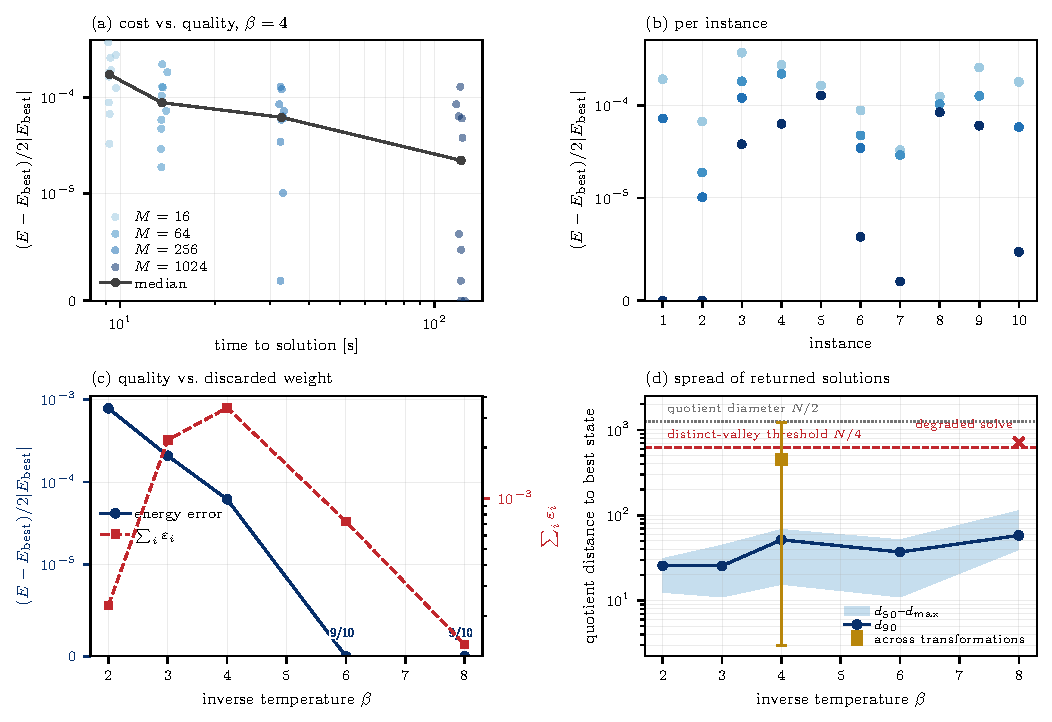
\includegraphics[width=\linewidth]{figures/quality.pdf}
\caption{Ten 2500-spin ($50\times50$) square-lattice instances at bond dimension 8,
on CPU. (a) Time to solution against relative energy error as the search breadth
$M=$~\texttt{max\_states} varies over $16$--$1024$; points are individual instances,
the line their median. (b) The same runs resolved per instance. (c) Median energy
error and median discarded weight $\sum_i\varepsilon_i$ against $\beta$;
annotations count instances reaching the best energy found. $E_{\mathrm{best}}$ is
the lowest energy over all settings here, not a certified optimum, so a zero error
means ``best found'', not ``optimal''. The two curves in (c) diverge: quality
improves monotonically with $\beta$ while discarded weight peaks at $\beta=4$ and
then falls. (d) How far apart the returned solutions actually are, at $M=1024$.
These instances carry no local fields, so $E(\sigma)=E(-\sigma)$ exactly and every
state has a degenerate mirror at Hamming distance $N$; distances are therefore
quotient distances $\min(d,N-d)$, on a space of diameter $N/2$. Band and line are
medians over the ten instances of the $50$th, $90$th and $100$th percentile of the
distance from each returned state to the best one. The whole returned set is a
single tight cluster, one to two orders of magnitude below the $N/4$ threshold a
diversity count would apply. The one point clearing it ($\beta=8$, instance 1) is a
degraded contraction --- its energy is $8$ above that instance's best and it fails
to return even the exact mirror --- not a second optimum. The square marker asks the
same question across contraction orders instead: one state from each of the eight
lattice transformations, $\beta=4$, median over five instances of the pairwise
minimum, median and maximum. Eight states from eight orders span the configuration
space; $1024$ states from one order do not.}
\label{fig:evr}
\end{figure}

\begin{figure}[t]
\centering
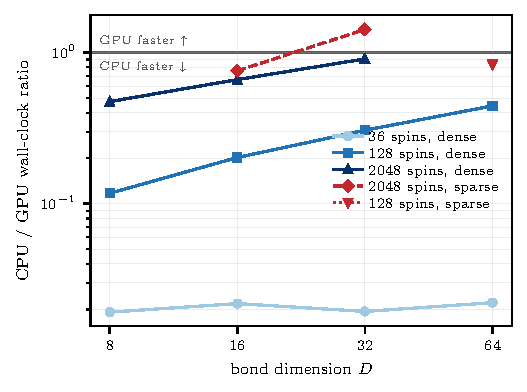
\includegraphics[width=0.62\linewidth]{figures/crossover.pdf}
\caption{Where GPU execution begins to pay: CPU/GPU wall-clock ratio on identical
configurations, so values below one mean the host is faster. The device wins only
once both the instance and the bond dimension are large. Data as in
Table~\ref{tab:cross}.}
\label{fig:cross}
\end{figure}

\textbf{When the GPU is worth using.} The original article recommends the GPU for
its larger examples without qualification. Solving identical configurations on each
device (Figure~\ref{fig:cross}, Table~\ref{tab:cross}) shows that holds only above a
threshold easy to fall below: the host is ${\approx}45\times$ faster at 36 spins
and, at 2048 spins and bond 16, still ${\approx}1.6\times$ faster in the dense case
(${\approx}1.3\times$ sparse); the device overtakes it only in the largest
sparse case --- 2048 spins at bond 32, where the GPU is ${\approx}1.4\times$ faster;
the dense case at that size still favours the host by ${\approx}10\%$. Energies agree
in every cell. Exploratory work therefore belongs on the CPU; the D-Wave-scale sparse
regime at large bond is where the device earns its place.

\begin{table}[t]
\small
\centering
\caption{Data behind Figure~\ref{fig:cross}: host versus device on identical
configurations, as CPU/GPU wall-clock ratio (below 1 means the CPU is faster). `Zipper', `SquareSingleNode',
$\beta{=}3$, \texttt{max\_states}${=}128$ throughout; separate alternating
processes on the H100 server (Intel Xeon Platinum 8462Y+, one NVIDIA H100).}
\label{tab:cross}
\begin{tabular}{@{}lcccc@{}}
\toprule
Spins & $D{=}8$ & $D{=}16$ & $D{=}32$ & $D{=}64$ \\
\midrule
36 (dense)     & 0.02 & 0.02 & 0.02 & 0.02 \\
128 (dense)    & 0.14 & 0.21 & 0.36 & 0.46 \\
128 (sparse)   & ---  & ---  & ---  & 0.68 \\
2048 (dense)   & 0.50 & 0.64 & 0.90 & --- \\
2048 (sparse)  & ---  & 0.78 & \textbf{1.45} & --- \\
\bottomrule
\end{tabular}
\end{table}

\begin{figure}[t]
\centering
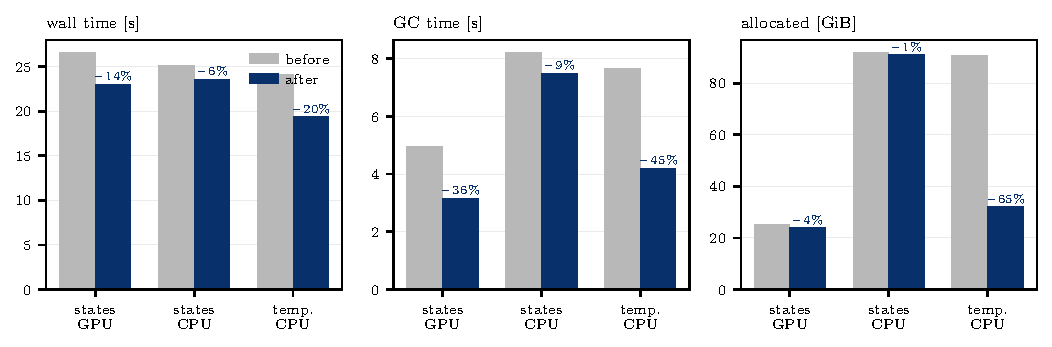
\includegraphics[width=\linewidth]{figures/allocation.pdf}
\caption{Allocated memory before and after the two allocation changes, on a
2048-spin bond-32 solve; percentages are the reduction. ``states'' is the
matrix-backed branched configuration set, ``temp.'' the off-heap contraction
temporaries. The temporaries change removes about two-thirds of the CPU heap; the
states change is small in \emph{bytes} because its benefit is a reduced live-object
count rather than volume. Allocated bytes are hardware-independent --- the H100 run
reproduces the post-change figures (32.3~GiB CPU, 24.1~GiB GPU).}
\label{fig:alloc}
\end{figure}

\textbf{Where the time actually goes.} Profiling explains both tables and
redirects the obvious optimizations. The device is never the constraint: on a
profiled 128-spin solve, host-side CUDA API calls account for only about a quarter
of wall time and the majority is host-side Julia work. The solver is host-bound at
every size we measured --- which is why the CPU stays competitive with the device
across the crossover, the tensor work being nearly free but removing none of the
bookkeeping.

An idle device invites kernel-level batching, and we did not pursue it for a reason
worth recording: eliminating the entire CUDA API share would cap at
${\approx}1.3\times$, whereas the host allocation load was reachable directly. A
single line, \texttt{branch\_states} in the branch-and-bound search, accounted for
52.7\% of the bytes a solve allocated; two changes follow
(Figure~\ref{fig:alloc}). The branched-configuration set is now backed by a single
matrix rather than tens of thousands of small vectors per call, cutting the number
of live objects sharply --- its allocated \emph{bytes} fall only ${\approx}4\%$ on
the large solve, but the object count that drives collection falls far more.
Separately, the multi-tensor contraction temporaries were moved off the collected
heap onto explicit allocation, cutting a 2048-spin bond-32 solve's allocated bytes
by about two thirds (90.9 to 32~GiB on CPU). Both reductions are hardware-independent
--- the H100 run reproduces the post-change figures --- and both were measured in a
full solve, since the explicit allocator is no faster in isolation and pays only
through the allocations it removes from the collected heap.

\textbf{Impact, limitations and outlook.} Contraction error is now an observable
rather than an article of faith, letting a practitioner distinguish a converged run
from a broken one on a problem where no exact answer is available --- the regime the
method exists for --- provided it is read as a statement about the contraction and
not about solution quality. The consolidation and the deprecation shims make the
published interface reproducible, and shipping the benchmark instances closes a gap
in that reproducibility that predates this update. The raw per-run data and figure
scripts behind the figures and tables, together with runnable drivers for the
crossover, concurrency, diversity, energy-vs-runtime, contraction-error, and
$\beta$-ladder results, are provided with the manuscript sources in the
\texttt{benchmarks/} directory. The allocation figure reports allocated bytes,
which are hardware-independent; the H100 run reproduces its post-change values,
and its pre-change values are recorded measurements of the superseded code.

The limitations are equally plain. Warm starting and the
discarded-weight measure cannot be combined, and warm starting currently covers only
the bottom boundary MPS, so layouts that build the top boundary do not benefit on
those rows. The error measure answers a narrower question than one might hope: it
bounds what the contraction discarded, and our own attempt to use it to select
$\beta$ failed, which is why the package now documents it as a diagnostic rather
than a criterion.

The remaining headroom is host-side rather than in the tensor kernels. The
branch-and-bound bookkeeping still dominates allocation even after the change above,
and the sparse contraction path --- which is where the device wins, per
Table~\ref{tab:cross} --- has not received the allocator treatment the dense one now
has. Both are more promising than the batching the idle device superficially
suggests.

\section*{Acknowledgements}
\label{acknowledgements}

This work was supported by the National Science Center (NCN), Poland, via
project Sonata Bis 10, No.~2020/38/E/ST3/00269 (B.G.), and Sonata Bis 15,
No.~2025/58/E/ST6/00422 ({\L}.P.).

\bibliographystyle{elsarticle-num}
\bibliography{refs}

\end{document}
